%%%%%%%%%%%%%%%%%%%%%%%%%%%%%%%%%%%%%%%%%
% Journal Article
% LaTeX Template
% Version 1.3 (9/9/13)
%
% This template has been downloaded from:
% http://www.LaTeXTemplates.com
%
% Original author:
% Frits Wenneker (http://www.howtotex.com)
%
% License:
% CC BY-NC-SA 3.0 (http://creativecommons.org/licenses/by-nc-sa/3.0/)
%
%%%%%%%%%%%%%%%%%%%%%%%%%%%%%%%%%%%%%%%%%

%----------------------------------------------------------------------------------------
%	PACKAGES AND OTHER DOCUMENT CONFIGURATIONS
%----------------------------------------------------------------------------------------

\documentclass[twoside]{article}

\usepackage{lipsum} % Package to generate dummy text throughout this template
%\usepackage[caption=false]{subfig}
%\captionsetup[subfigure]{labelformat=brace}
\usepackage{graphicx, bm} % Required to insert images
\usepackage[]{algorithm2e}
\usepackage{capt-of}%%To get the caption
\usepackage{listings} % Required for insertion of code
\usepackage[usenames,dvipsnames]{color} % Required for custom colors
\usepackage[sc]{mathpazo} % Use the Palatino font
\usepackage[T1]{fontenc} % Use 8-bit encoding that has 256 glyphs
\linespread{1.05} % Line spacing - Palatino needs more space between lines
\usepackage{microtype} % Slightly tweak font spacing for aesthetics

\usepackage{amsmath}
\usepackage{amssymb}

\usepackage[hmarginratio=1:1,top=32mm,columnsep=20pt]{geometry} % Document margins
\usepackage{multicol} % Used for the two-column layout of the document
\usepackage[hang, small,labelfont=bf,up,textfont=it,up]{caption} % Custom captions under/above floats in tables or figures
\usepackage{booktabs} % Horizontal rules in tables
\usepackage{float} % Required for tables and figures in the multi-column environment - they need to be placed in specific locations with the [H] (e.g. \begin{table}[H])
\usepackage{hyperref} % For hyperlinks in the PDF
\usepackage{subcaption}
\usepackage{lettrine} % The lettrine is the first enlarged letter at the beginning of the text
\usepackage{paralist} % Used for the compactitem environment which makes bullet points with less space between them
\usepackage{titlesec}
\usepackage{cancel}

\usepackage{abstract} % Allows abstract customization
\renewcommand{\abstractnamefont}{\normalfont\bfseries} % Set the "Abstract" text to bold
\renewcommand{\abstracttextfont}{\normalfont\small\itshape} % Set the abstract itself to small italic text


\usepackage{fancyhdr} % Headers and footers
\pagestyle{fancy} % All pages have headers and footers
\fancyhead{} % Blank out the default header
\fancyfoot{} % Blank out the default footer
\fancyhead[C]{STAT-221: Project $\bullet$ December 2014} % Custom header text
\fancyfoot[RO,LE]{\thepage} % Custom footer text

%----------------------------------------------------------------------------------------
%	CODE INCLUSION CONFIGURATION
%----------------------------------------------------------------------------------------

\definecolor{MyDarkGreen}{rgb}{0.0,0.4,0.0} % This is the color used for comments
\lstloadlanguages{R} % Load Perl syntax for listings, for a list of other languages supported see: ftp://ftp.tex.ac.uk/tex-archive/macros/latex/contrib/listings/listings.pdf
\lstset{language=R, % Use Perl in this example
        frame=single, % Single frame around code
        basicstyle=\scriptsize\ttfamily, % Use small true type font
        keywordstyle=[1]\color{Blue}\bf, % Perl functions bold and blue
        keywordstyle=[2]\color{Purple}, % Perl function arguments purple
        keywordstyle=[3]\color{Blue}\underbar, % Custom functions underlined and blue
        identifierstyle=, % Nothing special about identifiers                                         
        commentstyle=\usefont{T1}{pcr}{m}{sl}\color{MyDarkGreen}\scriptsize, % Comments small dark green courier font
        stringstyle=\color{Purple}, % Strings are purple
        showstringspaces=false, % Don't put marks in string spaces
        tabsize=2, % 5 spaces per tab
        %
        % Put standard Perl functions not included in the default language here
        morekeywords={rand},
        %
        % Put Perl function parameters here
        morekeywords=[2]{on, off, interp},
        %
        % Put user defined functions here
        morekeywords=[3]{test},
       	%
        morecomment=[l][\color{Blue}]{...}, % Line continuation (...) like blue comment
        numbers=left, % Line numbers on left
        firstnumber=1, % Line numbers start with line 1
        numberstyle=\tiny\color{Blue}, % Line numbers are blue and small
        stepnumber=5 % Line numbers go in steps of 5
}

% Creates a new command to include a perl script, the first parameter is the filename of the script (without .pl), the second parameter is the caption
\newcommand{\Rscript}[2]{
\begin{itemize}
\item[]\lstinputlisting[caption=#2,label=#1]{#1.R}
\end{itemize}
}

%----------------------------------------------------------------------------------------
%	TITLE SECTION
%----------------------------------------------------------------------------------------

\title{\vspace{-15mm}\fontsize{24pt}{10pt}\selectfont\textbf{STAT-221: Project}} % Article title

\author{
\large
\textsc{Kevin Kuate Fodouop}\\ % Your name
\normalsize Harvard University \\ % Your institution
%\normalsize \href{mailto:john@smith.com}{john@smith.com} % Your email address
\vspace{-5mm}
}
\date{}

%----------------------------------------------------------------------------------------

\begin{document}

\maketitle % Insert title

\thispagestyle{fancy} % All pages have headers and footers

%----------------------------------------------------------------------------------------
%	ABSTRACT
%----------------------------------------------------------------------------------------

\begin{abstract}
The Ebola epidemics which has affected West Africa since March 2014 is the most dramatic since the discovery of the virus in 1976, and has generated deep attention and fear among the international community. On several aspects, the response of the WHO has been categorized as too slow or lacking the needed means \cite{ebolresp}. This paper attempts to examine subnational data in county touched by Ebola to categorize the intensity of a potential virus outbreak in the region (higher spread or lower spread). We adapt the Grade of Membership (GoM) model studied in Caldas de Castro et al. \cite{malaria}, and assess the relevance on our model based on a previous study of regional Ebola spread \cite{ebolpred}.
\end{abstract}

%----------------------------------------------------------------------------------------
%	ARTICLE CONTENTS
%----------------------------------------------------------------------------------------

%\begin{multicols}{2} % Two-column layout throughout the main article text

\section{Literature Review}

This project uses Grade of Membership (GoM) models, and is based on former a study of malaria epidemics using Mixed Membership Models (MMM) \cite{malaria}. The objective in \cite{malaria} is to categorize regions as high risk or low risk for malaria, and use this information to optimize allocation of resources to prevent the disease's spread.\\

MMM are a flexible clustering model, meaning that every point partially belongs to all clusters to a certain degree (in a similar manner as in fuzzy c-means clustering). If the number of cluster is $K$, each subject has a membership vector $g^{(i)} = (g^{(i)}_1, ..., g^{(i)}_K)$ (components adding to 1). The probability of observing a response variable $x^{(i)}_j$ for this subject, given $\theta_k$ parameters of the response distribution in each cluster, is $Pr(x^{(i)}_j | g^{(i)}) = \sum_k g^{(i)}_k f(x^{(i})_j | \theta_{k j})$ \cite{mixmem}.\\

The different variables in the response X are considered independent given the GoM score $g$. \cite{malaria} also assumes all variables are categorical, so that $\theta_{k j}$ will be parameters of a multinomial distribution with $n=1$. Having $K=2$, corresponding to low or high profiles, the likelihood for the model reduces to
\begin{equation}
\mathcal{L}(X, G, \Theta) = \prod_{i=1}^N \prod_{j=1}^P \left[ g_{L, i} \* \prod_{m = 1}^{d_j} (\theta_{L, j})_m^{1_{x^{(i)}_j = m}} + g_{H, i} \* \prod_{m = 1}^{d_j} (\theta_{H, j})_m^{1_{x^{(i)}_j = m}} \right]
\end{equation}
with $d_j$ the number of levels for feature $j$. The optimal GoM $g$ and distribution parameter $\theta$ is obtained by stepwise MLE, detailed in algorithm 1.

\vspace{.2 in}

\begin{algorithm}[H]
 \KwData{Observed categorical data $X$}
 \KwResult{MLE of parameter $\Theta$ and GoM $g$.}
 initialization: $g = g_0$, $\Theta = \Theta_0$ initial guesses (can be derived from former results).\\
 \While{$|\mathcal{L}(X, G^{(k)}, \Theta^{(k)}) - \mathcal{L}(X, G^{(k - 1)}, \Theta^{(k - 1)})| > \epsilon$}{
  - Update step: k = k + 1\\
  1. $G^{(k)} \leftarrow MLE(G)$ with other parameters fixed.\\
  2. $\Theta^{(k)_L} \leftarrow MLE(\Theta_L)$ with other parameters fixed.\\
  3. $\Theta^{(k)_H} \leftarrow MLE(\Theta_H)$ with other parameters fixed.\\
 }
 \caption{3 step MLE for GoM fitting.}
\end{algorithm}
\vspace{.2 in}

One main challenge of GoM model may be to determine the proper number of clusters K \cite{mixmemint}, but in \cite{malaria} it is inherently fixed at 2 by the objectives of the problem (predicting low or high profile of malaria risk). It is however less explicit to determine from which domains select variables for $X$, and how many level to defined for each of these variables. The categorization is indeed here more driven by "subject matter interpretations of meaningfully different levels of risk" more than on statistical cateogorization, such as quantiles. On that side, a novelty introduced by the paper is to distinguish two domains of features which will determine risk profiles, environmental features and behavioral/economic features.\\

Most importantly, the categorization is not based on the expected result of the clustering (malaria risk for \cite{malaria}, but on other variables that are likely to influence the result metric. To assess the quality of the resulting high-risk low-risk clustering, the authors of \cite{malaria} plot $g_{high}$ against the exposure-weighted malaria illness rate (EWR), which is a metric representing risk of malaria in the region.



\section{Application to Ebola Propagation}

The Ebola epidemics that broke out in March 2014 is still progressing at a steady rate in West Africa (more than 1,000 new cases a week). The 3 mainly affected countries are Guinea, Sirrea Leone and Liberia, which suffer from poor health infrastructures. After a few months of virus propagation, data on the epidemics is available, and organization such as Statistics without Borders have made them publicly available and standardized. This project explores the application of Grade of Membership (GoM) model fitted to geographic regional data to predict the speed of spread (\texttt{high-speed} or \texttt{low-speed}) after an Ebola outbreak in a region.\\

We adapt the Mixed Membership Models (MMM) introduced in \cite{mixmem}, and used in \cite{malaria} to predict the high or low risk of malaria propagation in regions of the Amazon. The actual low-speed or high-speed Ebola propagation is based on a former data science study of Ebola cases prediction \cite{ebolpred}. This project uses the SIR model, an epidemiology model for understanding complex dynamics of disease propagation systems \cite{sirwik}. Figure 1 shows 2 shapes of ebola cases and deaths time series. The SIR model computes estimates for contamination, recovery and death rates, and implies an exponential evolution of cumulative number of cases. Hence the region \texttt{GN-8} of Guinea would be suited for the SIR model, and categorized \texttt{high-speed}, whereas \texttt{GN-38} would be better fitted by an S-curve model, and is categorized \texttt{low-speed}.
\vspace{.1 in}

\begingroup
\centering
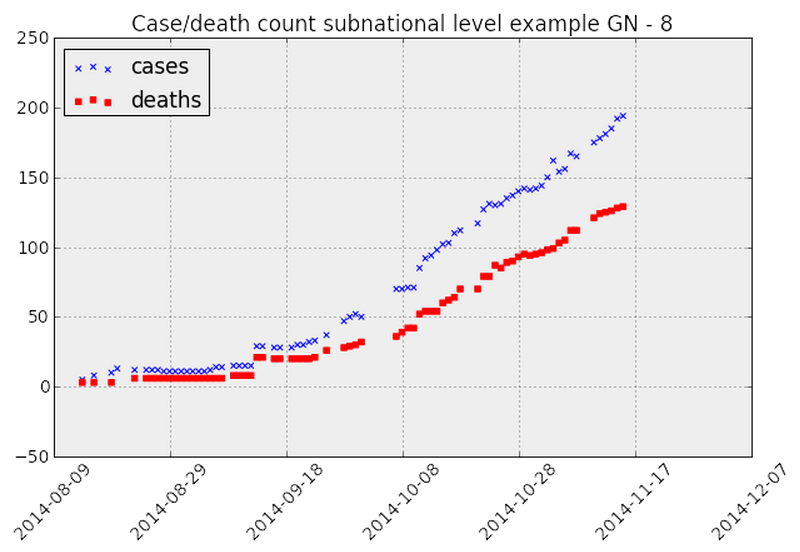
\includegraphics[scale=0.2]{./img/high_fit_cases.png}
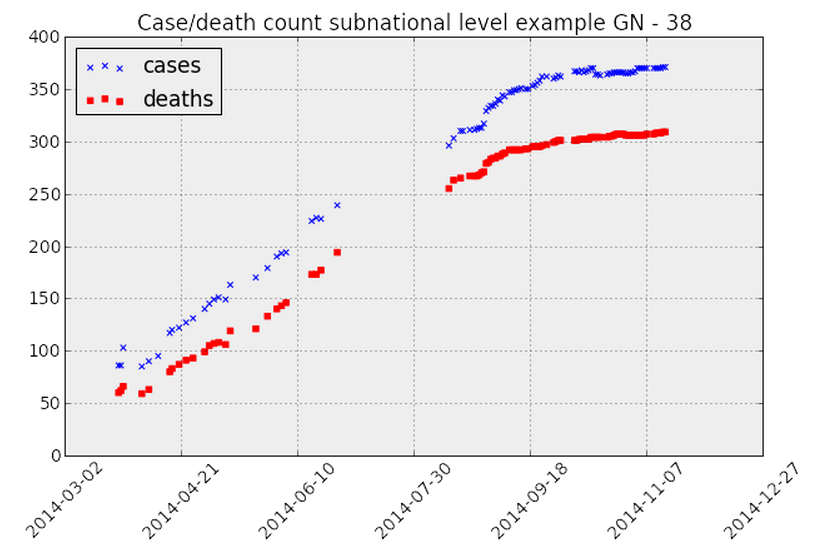
\includegraphics[scale=0.2]{./img/low_fit_case.png}
\captionof{figure}{Regions with cases shape adapted to SIR model (left), and not adapted to SIR model (right). Low model fit corresponds to a S-curve behavior, instead of exponential.}
\endgroup
\vspace{.2 in}

The SIR model only uses the cases (or deaths) time series data, and do not take into account regional features, such as quality of health infrastructures or access to clean water. Figure 2 displays a SIR fit for cases and deaths time series, for a region adapted to the model framework.

\vspace{.2 in}
\begingroup
\centering
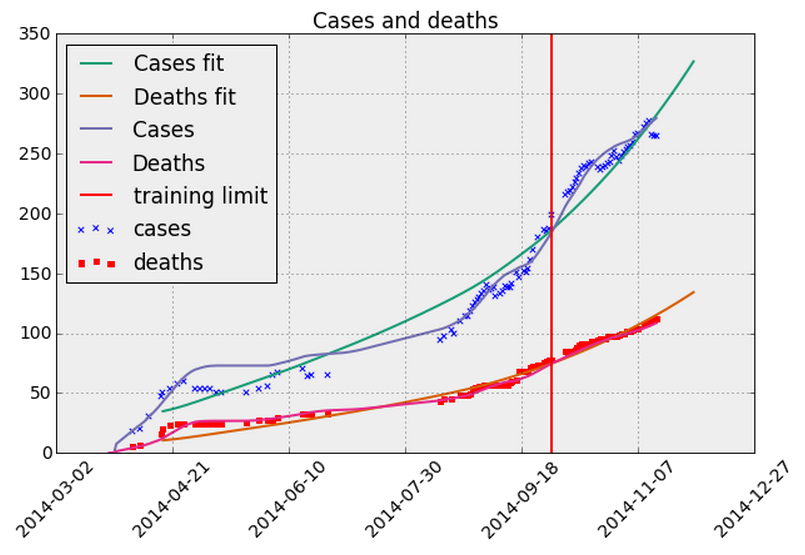
\includegraphics[scale=0.25]{./img/SIR_fit.png}
\captionof{figure}{Fit of the SIR model on a region showing exponential behavior in cases and deaths numbers.}
\endgroup

\vspace{.2 in}

The Ebola virus is transmitted to humans from wild animals, but then spreads in populations through human-to-human transmission. Reducing that human-to-human transmission is one the main objective of the WHO action \cite{ebolinfo}. The WHO action focuses on quick response to Ebola outbreaks, and acute monitoring of those outbreaks. However, few measures seem to be taken to preventively strengthen health infrastructures or sanitation procedures in region not yet touched by Ebola, but which would suffer fast propagation of the virus \cite{ebolresp}. The goal of this project is to use GoM models to predict the intensity of potential future outbreaks for that purpose.\\

As in \cite{malaria}, we use categorical features, and obtain a likelihood function of the form (1). The main challenge was to assess which variables to include in the model, and how to define the corresponding categories (starting with the number of such categories). Lacking the empirical research and subject matter expertise on feature importance for disease propagation, we adopted a statistically driven approach for the definition of such categories. For a defined number of categories, levels are computed comparing the observed value to the quantiles on the observations. The definition of such features to be included and their number of level is called a \textit{spread profile schema}.\\

To assess the quality of a \textit{spread profile schema}, we compute a commonly used goodness of fit metric for the resulting clustering, defined as
\begin{equation}
R_{clust} = \frac{sep_{inter}}{var_{intra}}
\end{equation}
$sep_{inter}$ being the inter-centroidal separation and $var_{intra}$ the intra-cluster variance. An adapted metric for fuzzy clustering is also computed. Results for some \textit{spread profile strucure} are documented in Table 1.\\

As a way to obtain the optimal \textit{spread profile schema} for our problem, we tried implementing a Genetic Algorithm method. Its chromosome structure encodes the number of levels for each features, and its fitness function is the clustering goodness of fit defined in (2) (fuzzy version). However we failed to define a crossover function that would efficiently explore the relevant chromosome space.\\

Adapting figure 2 of \cite{malaria}, we ploted GoM versus R-square obtained with the SIR model, grouped by country. Plots for bicategory (all category have 2 levels) schema is displayed on figure 3.

\vspace{.2 in}
\begingroup
\centering
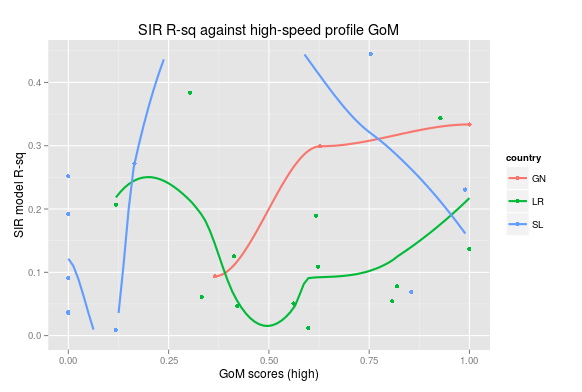
\includegraphics[scale=0.35]{./img/gom_rsq_bicat.png}
\captionof{figure}{Subareas SIR model fit ($R^2$) as a function of GoM scores (degree of belonging to \texttt{high-speed}).}
\endgroup

\section{Implementation}

Features were obtained from different sources, mainly the qDatum public sources repository on Ebola \cite{source}. Preprocessing and merging from the several sources was needed before obtaining the final features data in \texttt{dat/merged\_covariate\_df.csv}.\\
\indent
The results of SIR model fits is found in \texttt{dat/SIR\_fit.csv}. It contains $R^2$, $MSE$ goodness of fit metrics, and the number of observations. For assessing the relevance of our clustering results, we use the $R^2$ metric.\\

The structure of the code is as follows:
\begin{itemize}
\item \texttt{dat\_format.R}: Helper functions to convert data in the relevant categorical format, having specified features to be included and number of levels.
\item \texttt{MLE.R}: Functions performing the MLE optimization.
\item \texttt{SIR\_fit.R}: Functions to assess the quality of a clustering result and plot metric against GoM $g$, given the SIR regional fits.
\item \texttt{local\_optim.R}: Test GoM model locally, on first spread profile schemas. Also computes the matrix of suggested schemas to be tried on Odyssey.
\item \texttt{local\_ga.R}: Attempt to use Genetic Algorithm to determine best schema.
\item \texttt{schemas.R}: Data visualization of some feature distributions, and compute the schemas to be tried on Odyssey.
\item \texttt{mle\_task.R}: Try 100 schemas on 10 machines with Odyssey, triggered by \texttt{sbatch --array=1-10 mle.slurm}.
\end{itemize}

To perform the constraint optimization on the $\theta$s, we use the tranformation between the simplex and $\mathcal{R}^{d_p}$:
\begin{align*}
\xi_j = g(u_j) = log(u_j) - \sum_{j=1}^{d_p} log(u_j), \quad u_j = h(\xi_j) = \frac{e^{\xi_j}}{\sum_{j-1}^{d_p} e^{\xi_j}}
\end{align*}
$u$ being a column of one $\theta_p$, for low or high profiles. We have $h(g(u_j)) = u_i$. After transformation we can use R's \texttt{optim} function to perform the log-likelihood maximizations for the different steps described in algorithm 1.\\

The advantage of this design is that it makes it very easy to change the \textit{spread profile schema} (just change arguments of functions in \texttt{dat\_format.R}, and then assess the quality of the model. One direct drawback from this implementation, refering to \cite{mixmemint}, is that the categorization only relies on statistical quantiles, whereas subject specific empirical knowledge would be preferable. Hence even though it did not succeed, the motivation itself of the Genetic Algorithm approach can be challenged (as exogeneously derived categories would be better according to \cite{mixmemint}).


\section{Conclusion}

%----------------------------------------------------------------------------------------

%\end{multicols}

\clearpage
\begin{thebibliography}{9}
\bibitem{ebolinfo} \emph{Ebola Virus Disease,}
 by WHO Media Centre. 
\bibitem{ebolresp} \emph{Ebola Response Roadmap,} by 
	 WHO.
\bibitem{ebolpred} \emph{Predict Ebola!,} by 
	 Kristen Altenburger, Manuel Andere, Guillaume Sabran, and Shiya Wang.
\bibitem{sirwik} \emph{Compartmental models in epidemiology,} by 
	 Wikipedia. 
\bibitem{malaria}
	\emph{Malaria Risk on the Amazon Frontier,} by Marcia Caldas de Castro, Roberto L. Monte-Mor, Diana O. Sawyer, and Burton H. Singer.
\bibitem{mixmem}  \emph{Introduction to Mixed Membership Models and Methods,} by Edoardo M. Airoldi, David M. Blei, Elena A. Erosheva, Stephen E. Fienberg.
\bibitem{mixmemint}  \emph{Interpretability Contraints and Trade-offs in Using Mixed Membership Models,} by Burton H. Singer, Marcia C. Castro.
\bibitem{source}  \emph{http://www.qdatum.io/public-sources,} by qDatum.

\end{thebibliography}

\end{document}
